\documentclass[11pt]{article}

% Any additional packages needed should be included after jmlr2e.
% Note that jmlr2e.sty includes epsfig, amssymb, natbib and graphicx,
% and defines many common macros, such as 'proof' and 'example'.
%
% It also sets the bibliographystyle to plainnat; for more information on
% natbib citation styles, see the natbib documentation, a copy of which
% is archived at http://www.jmlr.org/format/natbib.pdf

\usepackage{jmlr2e}
\usepackage{hyperref}
\usepackage{bookmark}
\usepackage{multicol}
\usepackage{setspace} \doublespacing

% todonotes
\usepackage{xargs}                      % Use more than one optional parameter in a new commands
\usepackage[pdftex,dvipsnames]{xcolor}  % Coloured text etc.
\usepackage[colorinlistoftodos,prependcaption,textsize=tiny]{todonotes}
\newcommandx{\unsure}[2][1=]{\todo[linecolor=blue,backgroundcolor=blue!25,bordercolor=blue,#1]{#2}}
\newcommandx{\change}[2][1=]{\todo[linecolor=red,backgroundcolor=red!25,bordercolor=red,#1]{#2}}
\newcommandx{\info}[2][1=]{\todo[linecolor=OliveGreen,backgroundcolor=OliveGreen!25,bordercolor=OliveGreen,#1]{#2}}
\newcommandx{\improvement}[2][1=]{\todo[linecolor=Plum,backgroundcolor=Plum!25,bordercolor=Plum,#1]{#2}}
\newcommandx{\thiswillnotshow}[2][1=]{\todo[disable,#1]{#2}}

% margins for todonotes
\paperwidth=\dimexpr \paperwidth + 6cm\relax
\oddsidemargin=\dimexpr\oddsidemargin + 3cm\relax
\evensidemargin=\dimexpr\evensidemargin + 3cm\relax
\marginparwidth=\dimexpr \marginparwidth + 3cm\relax

% Definitions of handy macros can go here
\usepackage{subfig}
\newcommand{\dataset}{{\cal D}}
\newcommand{\fracpartial}[2]{\frac{\partial #1}{\partial  #2}}

\renewcommand*\contentsname{Table of Contents}

\begin{document}
\title{Syllabify and Conquer: A report on preparing and analysing speech text corpora}
\ShortHeadings{MSc. Project Report Winter 2022, McGill University}{}
\author{Author: Michael Haaf \textit{(michael.haaf@mail.mcgill.ca)} \\ Supervisor: Morgan Sonderegger \textit{(morgan.sonderegger@mcgill.ca)}}

\maketitle
\begin{singlespace}
\tableofcontents
\end{singlespace}
\newpage

\section{Introduction}

Natural language is a spoken phenomena, while the most common tools for computational natural language processing are predominantly text based. Tools that represent, store, and process audio signals associated with spoken natural language have not always existed and are not trivial to implement relative to comparable text-based processing tools. The reasons for this are straightforward: text-based data is comparably smaller in storage size and less demanding in memory to process. Moreover, speech-based data have much more complicated metadata and preprocessing requirements than text-based data; many of these complications put researcher out of the reach of amateur or non-technically proficient researchers. Speech transcription, aligning transcription with speech audio, audio signal processing, and non-uniform metadata/data storage standards are just some of the complications of speech-based natural language processing compared to text-based natural language processing. Given these obstacles, it is not surprising that more tools are researched, written, and developed for text-based corpora than for speech-based corpora in both natural language processing research and industry.

While the availability of speech-based corpora and automated tools to make use of them is increasing\cite{mcauliffe_polyglot_2017}, there remains a significant gap between the availability of speech data corpora and their general usability for researchers across disciplines. While libraries like NLTK\cite{noauthor_nltk_nodate} have bridged this gap with large accessible text-based natural language corpora and comprehensive tutorials for their usage, the same does not yet exist for speech data corpora.

This report documents work undertaken over a semester in the MCQLL Lab to perform experiments and develop software to help bridge this gap; particularly to the preparation problems of corpora storage and speech-text alignment. This project focused on the tools PolyglotDB\cite{mcauliffe_polyglot_2017} and Montreal Forced Aligner\cite{mcauliffe_montreal_nodate}, which respectively address the storage and alignment problems described. The aim of this project is to experiment and enhance these tools to extend their usability among non-expert researchers. Throughout the project, tutorials of the experiment progress were reproduced and updated.\footnote{https://polyglotdb.readthedocs.io/en/latest/tutorial.html} Additionally, experiments using PolyglotDB to analyze formants in a publicly available data set were performed successfully and documented in this report, to be published as tutorials in the near future. Overall summary of the deliverables and results of these efforts are elaborated in \hyperlink{section.5}{Section 5}.

The goal of increasing the accessibility of speech-data corpora software was addressed by performing experiments using publicly available corpora, and documenting steps taken to use these tools for facilitation of a pipeline from these public corpora to concrete linguistic analysis. These experiments, which demonstrate the ability to take public corpora and to answer interesting research questions, are verified experimentally and documented in \hyperlink{section.3}{Section 3} of this report. This report constitutes a technical description of work undertaken with these tools for reproduction, reuse, and as a basis for streamlining the investigation of more advanced linguistics problems that require similar speech data preparation and analysis techniques.

In \hyperlink{section.4}{Section 4}, this report additionally describes the software design approaches taken throughout the experimental process to implement a generalizable system for performing analysis on new corpora while minimizing coding changes needed. These approaches culminated in the contribution of tools written by the author and made available in a public repository\footnote{https://github.com/michaelhaaf/mfa-workbook}, that are technically documented in this report for future users, experimenters and developers. Alongside PolyglotDB and Montreal Forced Aligner, these tools facilitate the generalization of the experimental procedure taken across corpora and languages beyond those covered in the report experiments. This generalization is accomplished by abstracting the differences between corpora (varied in format and language) to a set of configuration files adaptable to the requirements of large sets of known public corpora. Differences in corpora that cannot be abstracted to configuration, especially syllabic differences in syllable representation across languages, are implemented using a Strategy pattern-based approach. This approach, dubbed ``syllabifying" in this report, streamlines the introduction of new client logic for new corpora to the adaptation of a testable and flexible template class. This approach aims to contribute a code-base that can dynamically adapt to and reliably implement future client requirements when new corpora necessitate novel business logic in configuration and linguistic structure.

The design approach described emerged from the set of challenging problems produced by the varied and rich nature of speech data corpora. These problems surround the automation of various steps in corpora preparation for storage, alignment, and analysis: transcript encoding, audio signal processing, and pronunciation dictionary convention generalization. These problems and their relation to the problems of speech data alignment, storage, and analysis are described in \hyperlink{section.2}{Section 2}, alongside discussion of the software contributed to resolve these problems and results indicating success in resolving them.

\section{Speech Data Preparation Pipeline}

While speech corpora are comprised of substantially the same basic elements across corpora and languages, speech corpora are also complex and heterogeneous in a variety of their features: metadata, directory structure, annotation files, documentation, for just some examples. Dozens of formats have been used to store speech corpora over the past several decades. These variations guarantee that workflow of getting general corpora ready for linguistic analysis is not homogeneous -- rather, complications introduced by these variations make manual workflows for general corpus work enormously labour-inducing. Researchers are often required to write scripts in order to make their workflow tenable.

For the research questions in this project, namely speech analysis of verb formants in spoken language across many speakers, it is assumed that an orthographic transcription of an audio file, time-aligned to the correct units of speech, is available to reliably associate sounds with known phonemes. This is not true of most publicly available speech corpora. Tools like Montreal Forced Aligner (MFA)\cite{mcauliffe_montreal_nodate} exist to force-align orthographic transcription files to their corresponding audio files. While the experiments conducted in \hyperlink{section.3}{Section 3} were already aligned at the beginning of the project (using MFA), there exist many other corpora that could be prepared for linguistic analysis in a similar manner. 

Currently, preparing data for usage with MFA usually involves manual scripting and organization of files. This is because the lexicon used by MFA to perform force alignment, and the lexicons documented in publicly available corpora, are never necessarily the same format, invoking the need to transform the metadata from one format to another. This creates classing parsing disambiguation problems to determine which token corresponds to which phoneme across pronunciation lexicon formats. To resolve these dynamic complications, and to pave the way for easier and more reliable extension to new corpora in the future, this project used Emergent Design Principles\cite{bain_emergent_2008} to adapt the generalizability of the code written as the complication of the requirements became more clear, revealing the natural application of the Strategy Pattern\cite{freeman_head_2004} to ``syllabify" pronunciation lexicons using configuration and extendable template classes. This work is documented in \hyperlink{section.4}{Section 4}.

The result is a speech data preparation pipeline from publicly available corpora to aligned speech-text corpora ready for analysis. Some examples demonstrated in this project are documented in this section. We make use of the publicly available IARPA BABEL corpora, particularly the Cantonese\cite{andrus_iarpa_2016} and Lithuanian\cite{benowitz_iarpa_2019} corpora, to demonstrate the procedure undertaken to prepare non-aligned corpora for linguistic analysis necessitating alignment.

The IARPA Babel Cantonese corpus contains scripted conversations recorded as audio files along with text file transcriptions of the conversations. Notably, the text files are not time-aligned with the .sph files, as they contain no time metadata at all. MFA is capable of time-aligning this corpora, but the file specifications for MFA are different than those for IARPA Babel; these differences are summarized in \hyperlink{table:corpus_format}{the table below.}\footnote{It should be noted that MFA does support automatic sampling frequency adjustments, and is not limited to 16kHz frequencies. 16kHz is the default, however, and we found that MFA performed better when the resampling took place in advance of the alignment.} 

\begin{table}[h!]
\centering
\begin{tabular}{|c|c c|} 
 \hline
 Corpus Parameter & MFA & IARPA Babel \\ [0.5ex] 
 \hline
 audio format & .wav & .sph \\
 sampling frequency & 16kHz & 8kHz \\
 transcript format & Praat\cite{noauthor_praat_nodate} TextGrid & .txt \\
\hline
\end{tabular}
\caption{This table summarizes some example configuration differences that occur between speech data corpora formats. Praat TextGrids are transcriptions which contain hierarchical time metadata. Additionally, this table does not include the difference in lexicon formats between the two corpora, though this is the most significant difference to adapt to -- these file types and analysis are developed further on in this section.}
\label{table:corpus_format}
\end{table}

The beginning task of the preparing corpora for alignment, then, is in part to convert corpora files to formats which MFA can recognize. Since natural language processing typically relies on large sample sets to draw reliable generalizations for automated tools, we are usually interested in large corpora, so these conversions should be implemented with an eye to perform efficiently at increasing scale.

In addition to file conversions, speech data corpora can differ significantly in their directory structures. The sample corpora chosen, the IARPA Babel Cantonese corpus, is compared below with the directory structure used by MFA.

\begin{multicols}{2}
\begin{singlespace}
\begin{verbatim}
IARPABabelCorpus/
|-- scripted/
|   |-- reference_materials/
|   |   |   lexicon.txt
|   |   |   lexicon.sub-train.txt
|   |-- training/
|   |   |-- audio/
|   |   |   |   recording1.sph
|   |   |   |   recording2.sph
|   |   |   |   ...
|   |   |-- transcript_roman/
|   |   |   |   recording1.txt
|   |   |   |   recording2.txt
|   |   |   |   ...
\end{verbatim}
\end{singlespace}

\begin{singlespace}
\begin{verbatim}
MFACorpus/
|   pronunciation_dictionary.txt
|-- textgrid_corpus/
|   |    recording1.wav
|   |    recording1.TextGrid
|   |    recording2.wav
|   |    recording2.TextGrid
|   |...






\end{verbatim}
\end{singlespace}
\end{multicols}

That is, the following steps need to be taken, while the resulting files should be stored in an MFA compatible directory structure:

\begin{singlespace}
\begin{itemize}
  \item Convert generic audio files to 16kHz .wav files
  \item Convert .txt transcripts to .TextGrid files, with all text contained in a single time hierarchy 
  \item Convert corpus lexicon to MFA-ready pronunciation dictionary
\end{itemize}
\end{singlespace}

This pipeline prepares generic speech-data corpora with orthographic audio recordings for conversion to an MFA ready format. The following subsections deal with each step of this pipeline in turn, making reference to code used and written throughout, and containing example results within each section.

\subsection{Speech Corpora Acquisition and Organization}

Two corpora sources were used in this study: IARPA Babel\cite{benowitz_iarpa_2019}\cite{andrus_iarpa_2016}, a US federal program to develop large-scale speech-data corpora for non English languages, as well as Librispeech test-clean\cite{panayotov_librispeech_2015}, a large-scale collection of dictated English speech. The corpora used ranged from 350MB to 890MB in total size, making these studies tractable for common development machines; part of the goal of this investigation is to determine if reliable and interesting analysis can be performant of data sets this small.

In this project, the IARPA Babel corpora have not been force aligned, and the goal of this project is to align them in preparation for linguistic analysis. For the Librispeech test-clean data set, a subset of the speakers have had this alignment preparation take place at the outset of the project; with some shell scripting, these speakers were filtered into a new data set for the experiments performed in \hyperlink{section.3}{Section 3}. To permit working in parallel on both tasks at the same time, this project made use of the already aligned subset of Librispeech, while preparing the two IARPA Babel corpora for analysis.

The rest of this section concerns the concrete preparation steps required to align the two IARPA Babel corpora.

\subsection{Transcript to TextGrid Conversion}

Generally, transcripts for audio corpora are not made available in a particular format. Most often, they are text files unadorned with particular metadata. Since force-alignment is a time-series categorization of data, however, there does need to be some representation of time in speech-text corpora for alignment to take place. One common known file specification that resolves this problem is the Praat\cite{noauthor_praat_nodate} TextGrid format. TextGrids allow for structuring ‘tiers’ into a text based file, allowing for a meaningful hierarchy for storage; for example, each phone token belongs to a corresponding word, and all phone tokens are considered events which take place within a given time range.

The conversion from general transcript files to TextGrids does not exist, since metadata and formatting can vary from transcript to transcript. This project makes use of the Python library praatio\cite{tim_mahrt_praatio_2016} which has useful utilities for performing this conversion. This project contributes a script, \verb|transcripts_to_textgrids.py|\footnote{https://github.com/michaelhaaf/mfa-workbook/blob/main/scripts/transcripts\_to\_textgrids.py}, which uses the praatio library to convert, in bulk, a directory of text transcript files. This approach also allows tuning the transcript file to remove unwanted tokens and to perform other useful preprocessing steps.

\subsection{Audio Signal Processing}

In addition to the text transcript files, the audio files of speech-text data corpora can vary in important properties. To align generic audio recordings with generic text transcriptions, there are two prerequisites: a known sampling frequency, and a known file format. As discussed in the preamble to this section, the Montreal Forced Aligner is used to perform force-alignments, which runs optimally using 16kHz sampling frequency and the .wav audio standard. While many other combinations of frequency and format are possible in principle, some standard must be applied in order for measurement to take place, in turn allowing automated alignment to take place. This section concerns the problem of transforming a large set of audio files to a common sampling frequency and a common file format standard.

For example, the IARPA corpus stores audio files using the .sph file format standard, with audio recorded at an 8kHz sample rate. This corpus therefore demonstrates a key example of a corpus needing transformations in both metrics. Conversion from this format to the MFA standard above requires scripting: while there exist many tools to convert and resample audio formats, there are none that, crucially, (1) convert arbitrary audio formats to a chosen standard (in this case, .wav); (2) resample .wav from arbitrary sampling frequency to a chosen standard (in this case, 16kHz) without altering the pitch nor speed of the audio file; (3) handle gigabytes of audio files in bulk without running into RAM issues on ordinary machines (16GB RAM).

By point of comparison, the Praat tool can do (1) and (2) but not (3), since Praat scripts, in an effort to produce a non-technical user experience, do not offer memory management or lazy/dynamic loading of audio files at runtime which would be required to fulfill requirement (3).

This project developed a method for performing all three tasks, by combining the Praat library, the sph2pipe\footnote{https://github.com/burrmill/sph2pipe} library , and intermediate shell scripting. The result is a script with user-friendly prompts and error messages which allows for specifying a directory of audio files to be converted and resampled according to specification at the command line. The shell script uses POSIX specified shell idioms (the \verb|find -exec| command pattern) to manage running expensive memory options on large-scale corpora without running out of memory while maximizing parallelization in processing. This project contributes a script\footnote{https://github.com/michaelhaaf/mfa-workbook/blob/main/scripts/bulk\_sph\_resample} which can be reused to perform similar audio signal processing on large directories in the future.

\subsection{Pronunciation Dictionary Production}

As discussed in a previous section, speech-text alignment matches sound to text tokenized upon phonemes. That is, an accurate alignment depends upon reliable decomposition of word pronunciations into constituent phonemes in the text layer. As such, MFA pronunciation dictionaries are two-column files, where the columns represent a one to many mapping from words to pronunciations, and where pronunciations are decomposed into syllables and constituent phonemes by token boundaries.

Speech data corpora under study in this project, such as the IARPA Babel corpus set, typically include a lexicon with a similar mapping as MFA. In the general case, however, the symbols and ordering of phonemes, and of syllabic structure, are nonstandard across corpora. A typical example follows:

\begin{multicols}{2}
  \begin{singlespace}
    IARPA Babel Cantonese Lexicon
    \begin{verbatim}
    meng2	m E: N _2
    m4chi5	m _4 . ts i: _5
    \end{verbatim}
  \end{singlespace}
  \begin{singlespace}
    MFA Pronunciation Dictionary
    \begin{verbatim}
    meng2	m E:2 N
    m4chi5	m4 ts i:5
    \end{verbatim}
  \end{singlespace}
\end{multicols}

That is, the word/pronunciation mapping from the IARPA Babel corpus is transformed to an MFA-compatible word/pronunciation mapping for each entry in the IARPA Babel lexicon. This is the general task of the pronunciation dictionary production phase of the speech data preparation pipeline.

In the example shown above, the problem appears to reduce to simple text manipulations to a standardized character set. The problem is inherently more complicated than this: close inspection of the examples above show that the ordering of tokens cannot be strictly assumed, especially when considering tones. Without phonological theory, the ordering of tokens cannot be determined accurately. A brief summary of the necessary syllable structure assumptions follows:\cite{fromkin_introduction_2006}:

Across languages, words are composed of one or more syllables, which are in turn composed of one or more phonemes. Every syllable has a nucleus, which is itself composed of one or more phonemes. Syllable nucleus may be preceded by one or more phonemes grouped together as an onset, and nucleus may be followed by one or more phonemes grouped together as a coda. Syllables may also have tone/stress indicators, paired with the nucleus vowel.

Further complications arise in determining the boundary between syllabic units. The nucleus may be the first token or the last, and it may itself be composed of more than one token. The bounds of the onset and the coda are dependent on the bounds of the nucleus. A general scheme for syllable unit determination follows:

\begin{itemize}
  \item Coda: all phonemes that occur before the first vowel in the syllable
  \item Nucleus: the first vowel in the syllable, followed by\begin{itemize}\item nothing\item a second vowel \item a sonorant\end{itemize}
  \item Coda: all phonemes that occur after the nucleus
  \item Tone: see below
\end{itemize}

Tone, as indicated above, is more complicated. In this project, tone was often ignored in the early stages in order to produce results faster. However, tone (and related information for non-tonal language: stress and pitch) are often included in publicly available corpora and are useful for more accurate alignment results to disambiguate important semantic and pragmatic content.

To demonstrate variation in tone, we can consider the IARPA Lithuanian corpus, compared with the IARPA Cantonese corpus we saw previously: \\

  \begin{singlespace}
    \noindent IARPA Babel Lithuanian Lexicon
    \begin{verbatim}
    Adomaitis   a . d o: . " m a_F I . t' I s
    \end{verbatim}
    MFA Pronunciation Dictionary
    \begin{verbatim}
    Adomaitis   a1 d o:1 m a5 I t' I1 s
    \end{verbatim}
  \end{singlespace}

  While we saw tone was marked explicitly in the Cantonese lexicon (although with an extra underscore token relative to the MFA format), in the Lithuanian lexicon tone is implicit -- this reflects that Lithuanian is not exactly a tonal language, but that there are 5 distinct stress markers which can be applied to Lithuanian syllables. These tone/stress markers are documented in the IARPA Babel Lithuanian corpus documentation\cite{benowitz_iarpa_2019}. 

  In the example above, third syllable is: \verb|" m a_F I|. This syllable is of immediate interest for demonstration. The \verb|_F| character indicates a falling accent, which combined with a long nucleus (composed of the vowels \verb|a| and \verb|I|), indicates that this syllable is a long vowel stressed with a falling accent, which according to the IARPA Babel Lithuanian corpus documentation, corresponds to the discrete tone category \verb|5|. This is just one example demonstrative of just some of the variation in complexity for tone and syllabic unit determination. 

While the structure of syllables is finite and tractable in scope, the variation in possible ordering and boundaries of phoneme tokens raises complications in simply reading tokens left to right to assign onset, nucleus, coda, and tone indicators. The software design approach to ``syllabifying", that is, translating pronunciations stored as text formats into data structures representing the phonetic structure of syllables, is described in \hyperlink{section.4}{Section 4: Software Design}.

The steps to produce a pronunciation dictionary for unifying the corpus formats (IARPA Babel and MFA) automatically, with potential easy extension for future corpora, is the primary contribution of the software written for this project. While more complicated than anticipated, these efforts were ultimately successful: the software reliably creates MFA-ready pronunciation dictionaries for the corpora under study (IARPA Lithuanian and IARPA Babel) from their input lexicons. 

Ultimately, the pronunciation dictionaries  we created now allow us to use MFA to produced aligned speech-text corpora.

\subsection{Alignment Production}

The goal of the force-alignment procedure is demonstrated by the figures below:

\begin{figure}[h]
\begin{minipage}[t]{.45\linewidth}
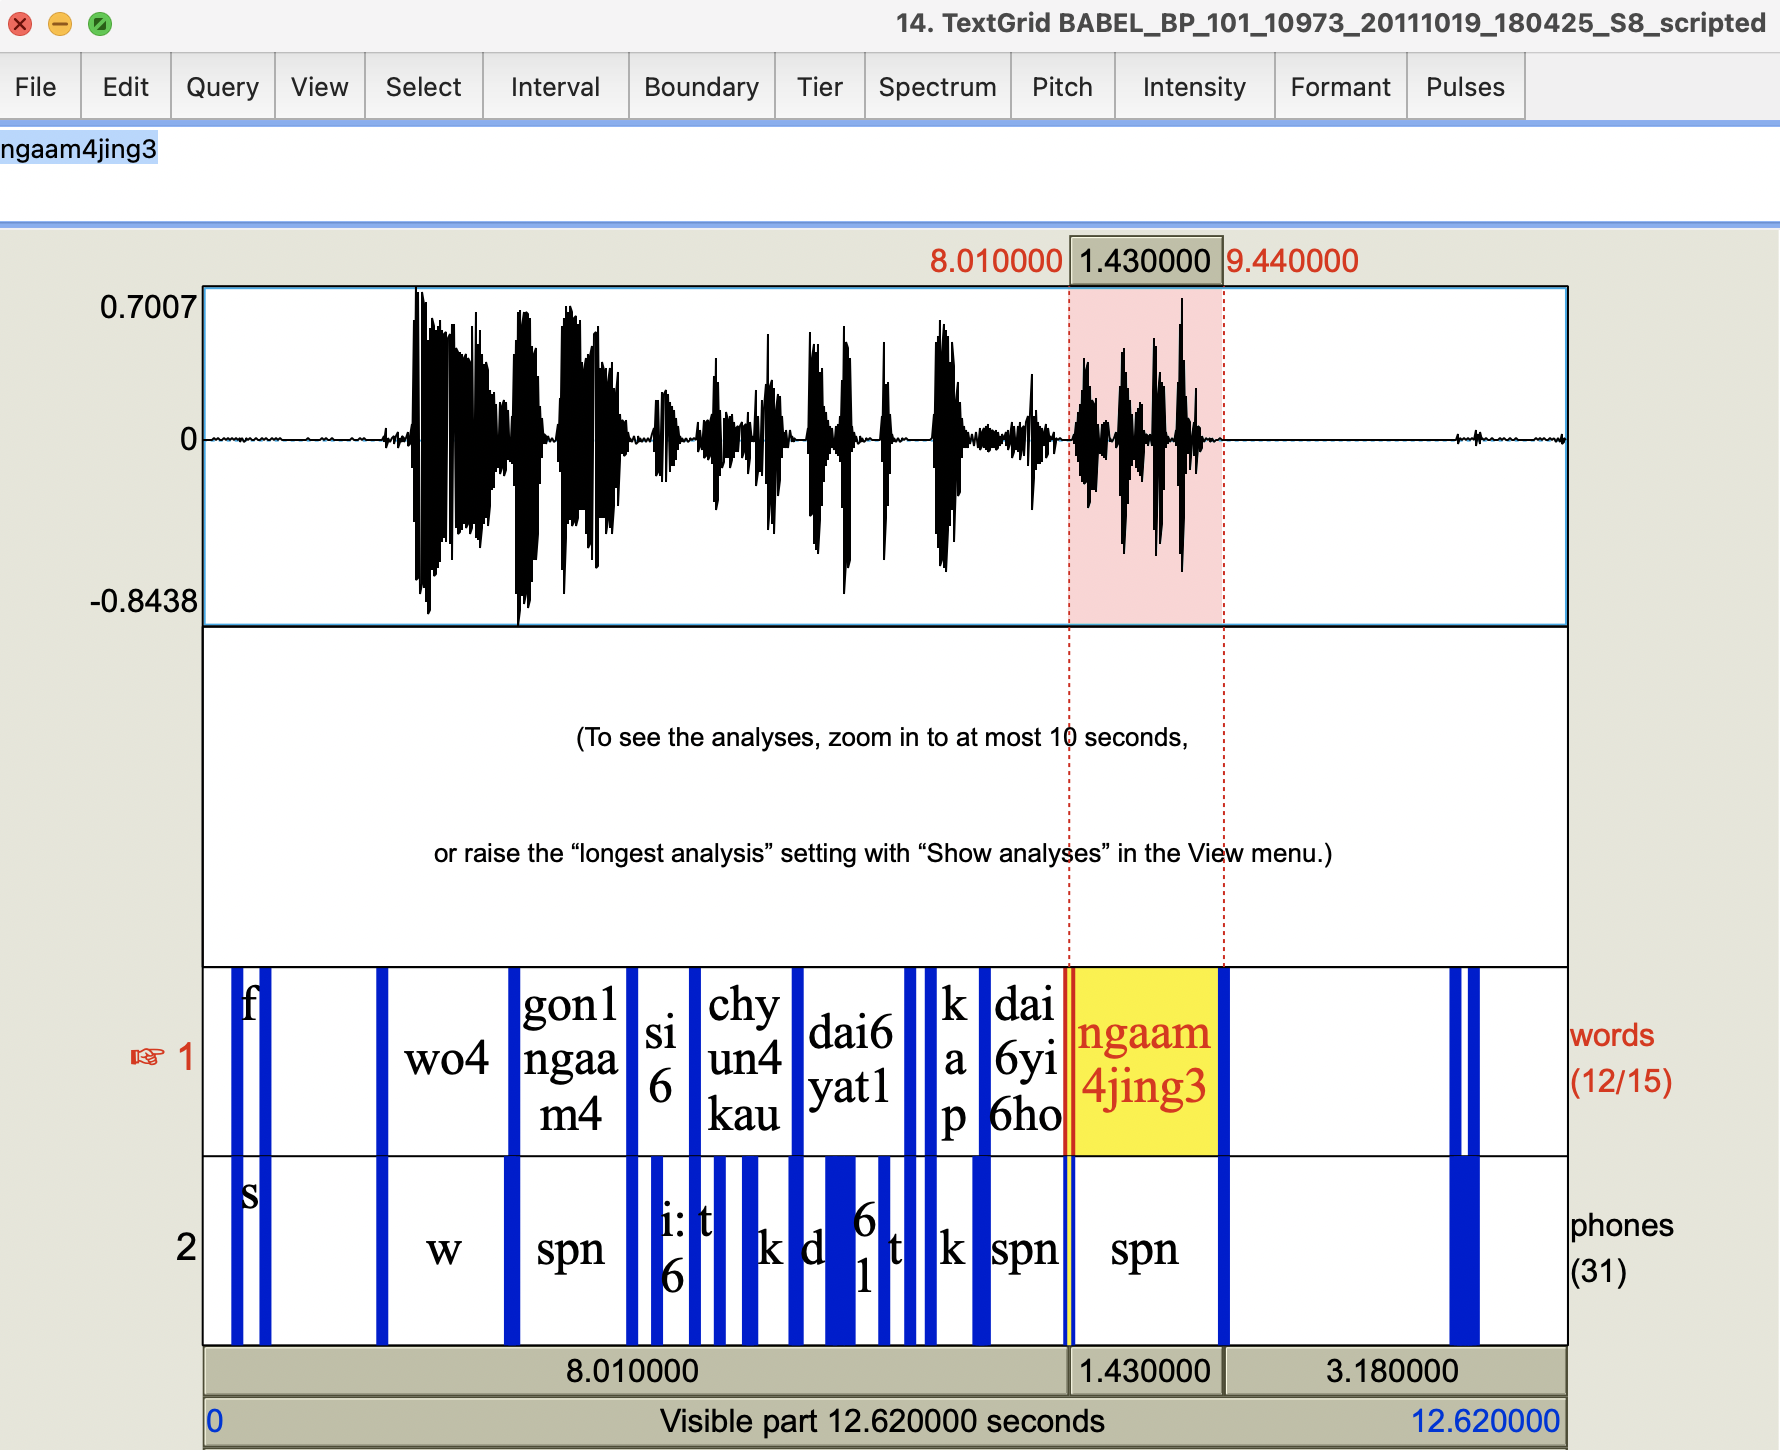
\includegraphics[width=\linewidth]{nonaligned.png}
\caption{An unsuccessful forced-alignment of a 12 second scripted recording} 
\end{minipage}\hfill
\begin{minipage}[b]{.45\linewidth}
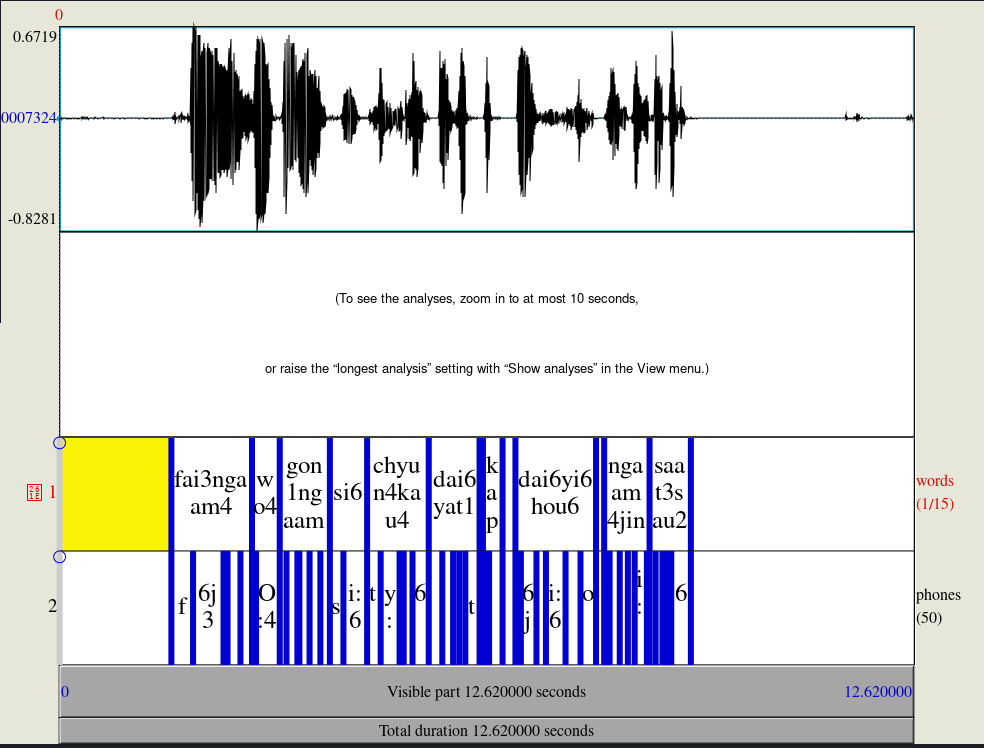
\includegraphics[width=\linewidth]{aligned.png}
\caption{A successful forced-alignment of the same 12 second scripted recording.} 
\end{minipage}
\end{figure}

Namely, the correct phonemes should be visibly matched with the corresponding audio signals. While there are automatic tools to detect out of vocabulary words and statistical measurements to the quality of alignment, a representative sample of alignments should be manually checked (and listened to) in order to verify that the force-alignment was carried out correctly.

In this project, the entire Cantonese IARPA set was aligned, and the Lithuanian set was aligned as well pending verification. For the Cantonese data set, out of roughly 16000 speaker files, there were roughly 650 files whose alignments failed, leaving just over 15000 which were aligned successfully according to available metrics and visual inspection of a subset of the data. This is important: losing more data to alignment errors prevents us from building a significant enough data set using which we can perform experiments.

\section{Experiments}

The previous section established a pipeline for turning publicly available corpora into aligned speech-text data sets ready for linguistic analysis. In parallel to producing this pipeline and applying it to the IARPA Babel Cantonese and Lithuanian corpora, this project also sought to reproduce basic linguistic analysis on aligned corpora to experiment with and extend the usability of the PolyglotDB platform.

This section outlines the process for taking aligned speech-text data sets. These data sets could be the aligned data sets produced in the pipeline (IARPA Cantonese and Lithuanian). In this case, the Librispeech test-clean data set, which had already been aligned prior to the experiment phase of this project, was used for these experiments. The process for acquiring the Librispeech test-clean aligned corpora is described in \hyperlink{section.21}{Section 2.1: Speech Corpora Acquisition}. The choice of this corpus both permitted parallel work on the data preparation pipeline, and facilitated easier comprehension of the linguistic analysis for general audiences, including the author himself.

This section begins with reproductions of existing PolyglotDB tutorials to demonstrate the basic mechanics of working with aligned corpora. It is followed by concrete investigation into basic linguistic research questions about the data set: for example, does the data set exhibit formant mappings typical of similar English speaker corpora? The production of these experiments, and discussion of their results, points the way to future more advanced linguistic analysis on these data sets and others that could be prepared by the speech data set pipeline discussed previously.

\subsection{PolyglotDB Package Management}

Before we move to the experiments performed, a quick note can be made about the development environment required to use these packages. PolyglotDB is a python package available for installation via pip, however, it does contain core dependencies that live outside of the python ecosystem; in particular, the NoSQL Java database library, InfluxDB. These dependencies can be varied in their support by general developer operating system platforms, and prior to this project, there was no one process that would automatically resolve these dependencies for a given PolyglotDB installation.

This project contributes a small procedure to automatically resolve system dependencies on all platforms that support Conda. The operation of this procedure is now described on the PolyglotDB website.\footnote{https://polyglotdb.readthedocs.io/en/latest/getting\_started.html\#conda-development-environment}

This project investigated a transition of the PolyglotDB platform from pip to modern python installation environments, such as condaforge\cite{conda_forge_community_2015_4774216}, where Montreal Forced Aligner is already available. Time constraints prevented this transition from being completed by the end of the semester, but progress is ongoing.\footnote{https://github.com/conda-forge/staged-recipes/pull/18313}

Condaforge support for PolyglotDB would allow for automatic management of python and Java dependencies on any machine that supports conda. Future work could investigate installation of PolyglotDB on new server architectures, such as the increasingly available ARM64 platform. For the time being, the procedure now provided on the PolyglotDB website linked in the footnote above is the procedure taken for the following experiments, and should be reproducible on most machines just like an automatic Conda installation. 

\subsection{Reproduction of Existing Experiments}

The problem of abstracting away manual scripting from performing linguistic analysis on an aligned speech-text corpora is addressed by PolyglotDB. To begin analysis, the corpora should be stored in a manner that allows reliable read/write querying for corpus investigation and enrichment. To facilitate this storage, this project followed existing PolyglotDB tutorials.\footnote{https://polyglotdb.readthedocs.io/en/latest/tutorial.html} This section overviews this process and summarizes the results.

As described in the \hyperlink{section.22}{Data Acquisition} section of this report, a forced-aligned Librispeech test-clean English data set was acquired from previous alignment efforts at MCQLL with basic shell scripting. While this data set is force-aligned with phonemes in time, there is no other interesting metadata associated with speakers. Associating speaker metadata (age, gender, residence, etc.) with speech data is an important component of speech data research. This section described the procedure for storing aligned data sets, and enriching them for linguistic analysis, by importing them into a PolyglotDB instance. 

PolyglotDB works by creating NoSQL time-series database in its development environment for speech data, and uses a SQL python library to wrap queries to speaker data stored in text files. Speech corpora can be imported and queried, with read/write permissions, using NoSQL under the hood, with queries wrapped in a python library for ease in interfacing with scripts and other software. Therefore, importing and enriching a corpora in a PolyglotDB database, then exporting the enriched corpora for analysis, can be done in a few lines of python, as shown in the tutorial. This tutorial was reproduced, with some typical examples of the kinds of queries that PolyglotDB supports.

Now that it has been established we can import, enrich, and make simple queries to a PolyglotDB instance, more interesting linguistic analysis can be performed.

\subsection{Formant Analysis}

Following the analysis preparation performed in the previous steps, in this section we process the output of the same Polyglot database we enriched, and show how it can be used to address basic linguistics research questions involving variation between speakers in vowel space.\footnote{Most of the analysis in this section was adapted from analysis done by Morgan Sonderegger (McGill), which itself is analysis is partly adapted from course materials by Márton Sóskuthy (UBC).} For example, we could verify basic aggregate properties of our data set by comparing vowel formant plots across speakers in our data set, or apply statistical analysis to investigate more interesting questions about properties of speaker dialects.

In this project, we carried out two such experiments: one to verify an expected property (do male speakers, on average, have lower vowel frequency utterances than female speakers?), and another to answer an interesting question about the speakers' dialects (which speakers exhibit the ``cot"--"caught" merger in their dialect?). This section explains our approach to addressing those questions with our corpus.

We begin with the exported data from the previous step: a .csv containing vowel formant measurements for each phoneme in the data set, associated with each speaker and speaker metadata. Some debugging in this step is required: forced-alignment is an automated, probabilistic process and like signal detection in general, will not make perfect predictions. Such alignment issues can carry over and be made visible by investigating timing/speech-rate calculation errors in particular. We carried out some sanitization measures data set manually: correcting columns with invalid values, filtering duration/F1/F2/standard deviation outliers, in order to a reliable subset given noisy measurements. These steps require some domain knowledge and scripting capability, but this is the beginning of the scientific investigation, so that is to be expected.

The filtered data set was reduced to about 3/5 its original size, to 43758 measurements from 74001, increasing the coherence of the formant measurements greatly. The filtered data set was happily significant enough to produce interesting results: we were able to observe coherent distinctions in speaker frequencies by sex, and in ``cot--caught" mergers by speaker dialect. These results are documented in the \hyperlink{fig:sex_formant}{figures} \hyperlink{fig:dialect-analysis}{below}.

    \begin{figure}[h]
      \centering
      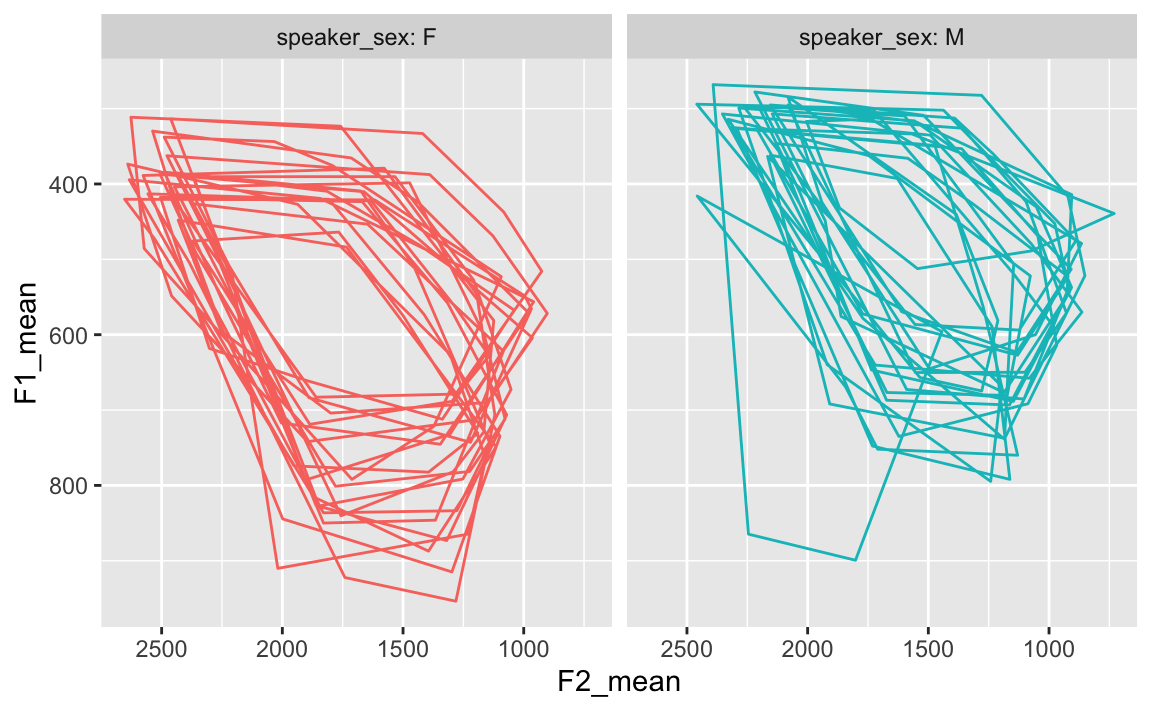
\includegraphics[scale=0.25]{sex_formant.png}
      \caption{Comparing the vowel formant plot of male and female speakers, the vowel space is noticeably shifted to lower F2 and F1 on average for male speakers compared to female speakers, verifying an expected result. Figure produced using code written by Morgan Sonderegger (McGill).}
      \label{fig:sex_formant}
    \end{figure}

    \begin{figure}[h]
      \centering
      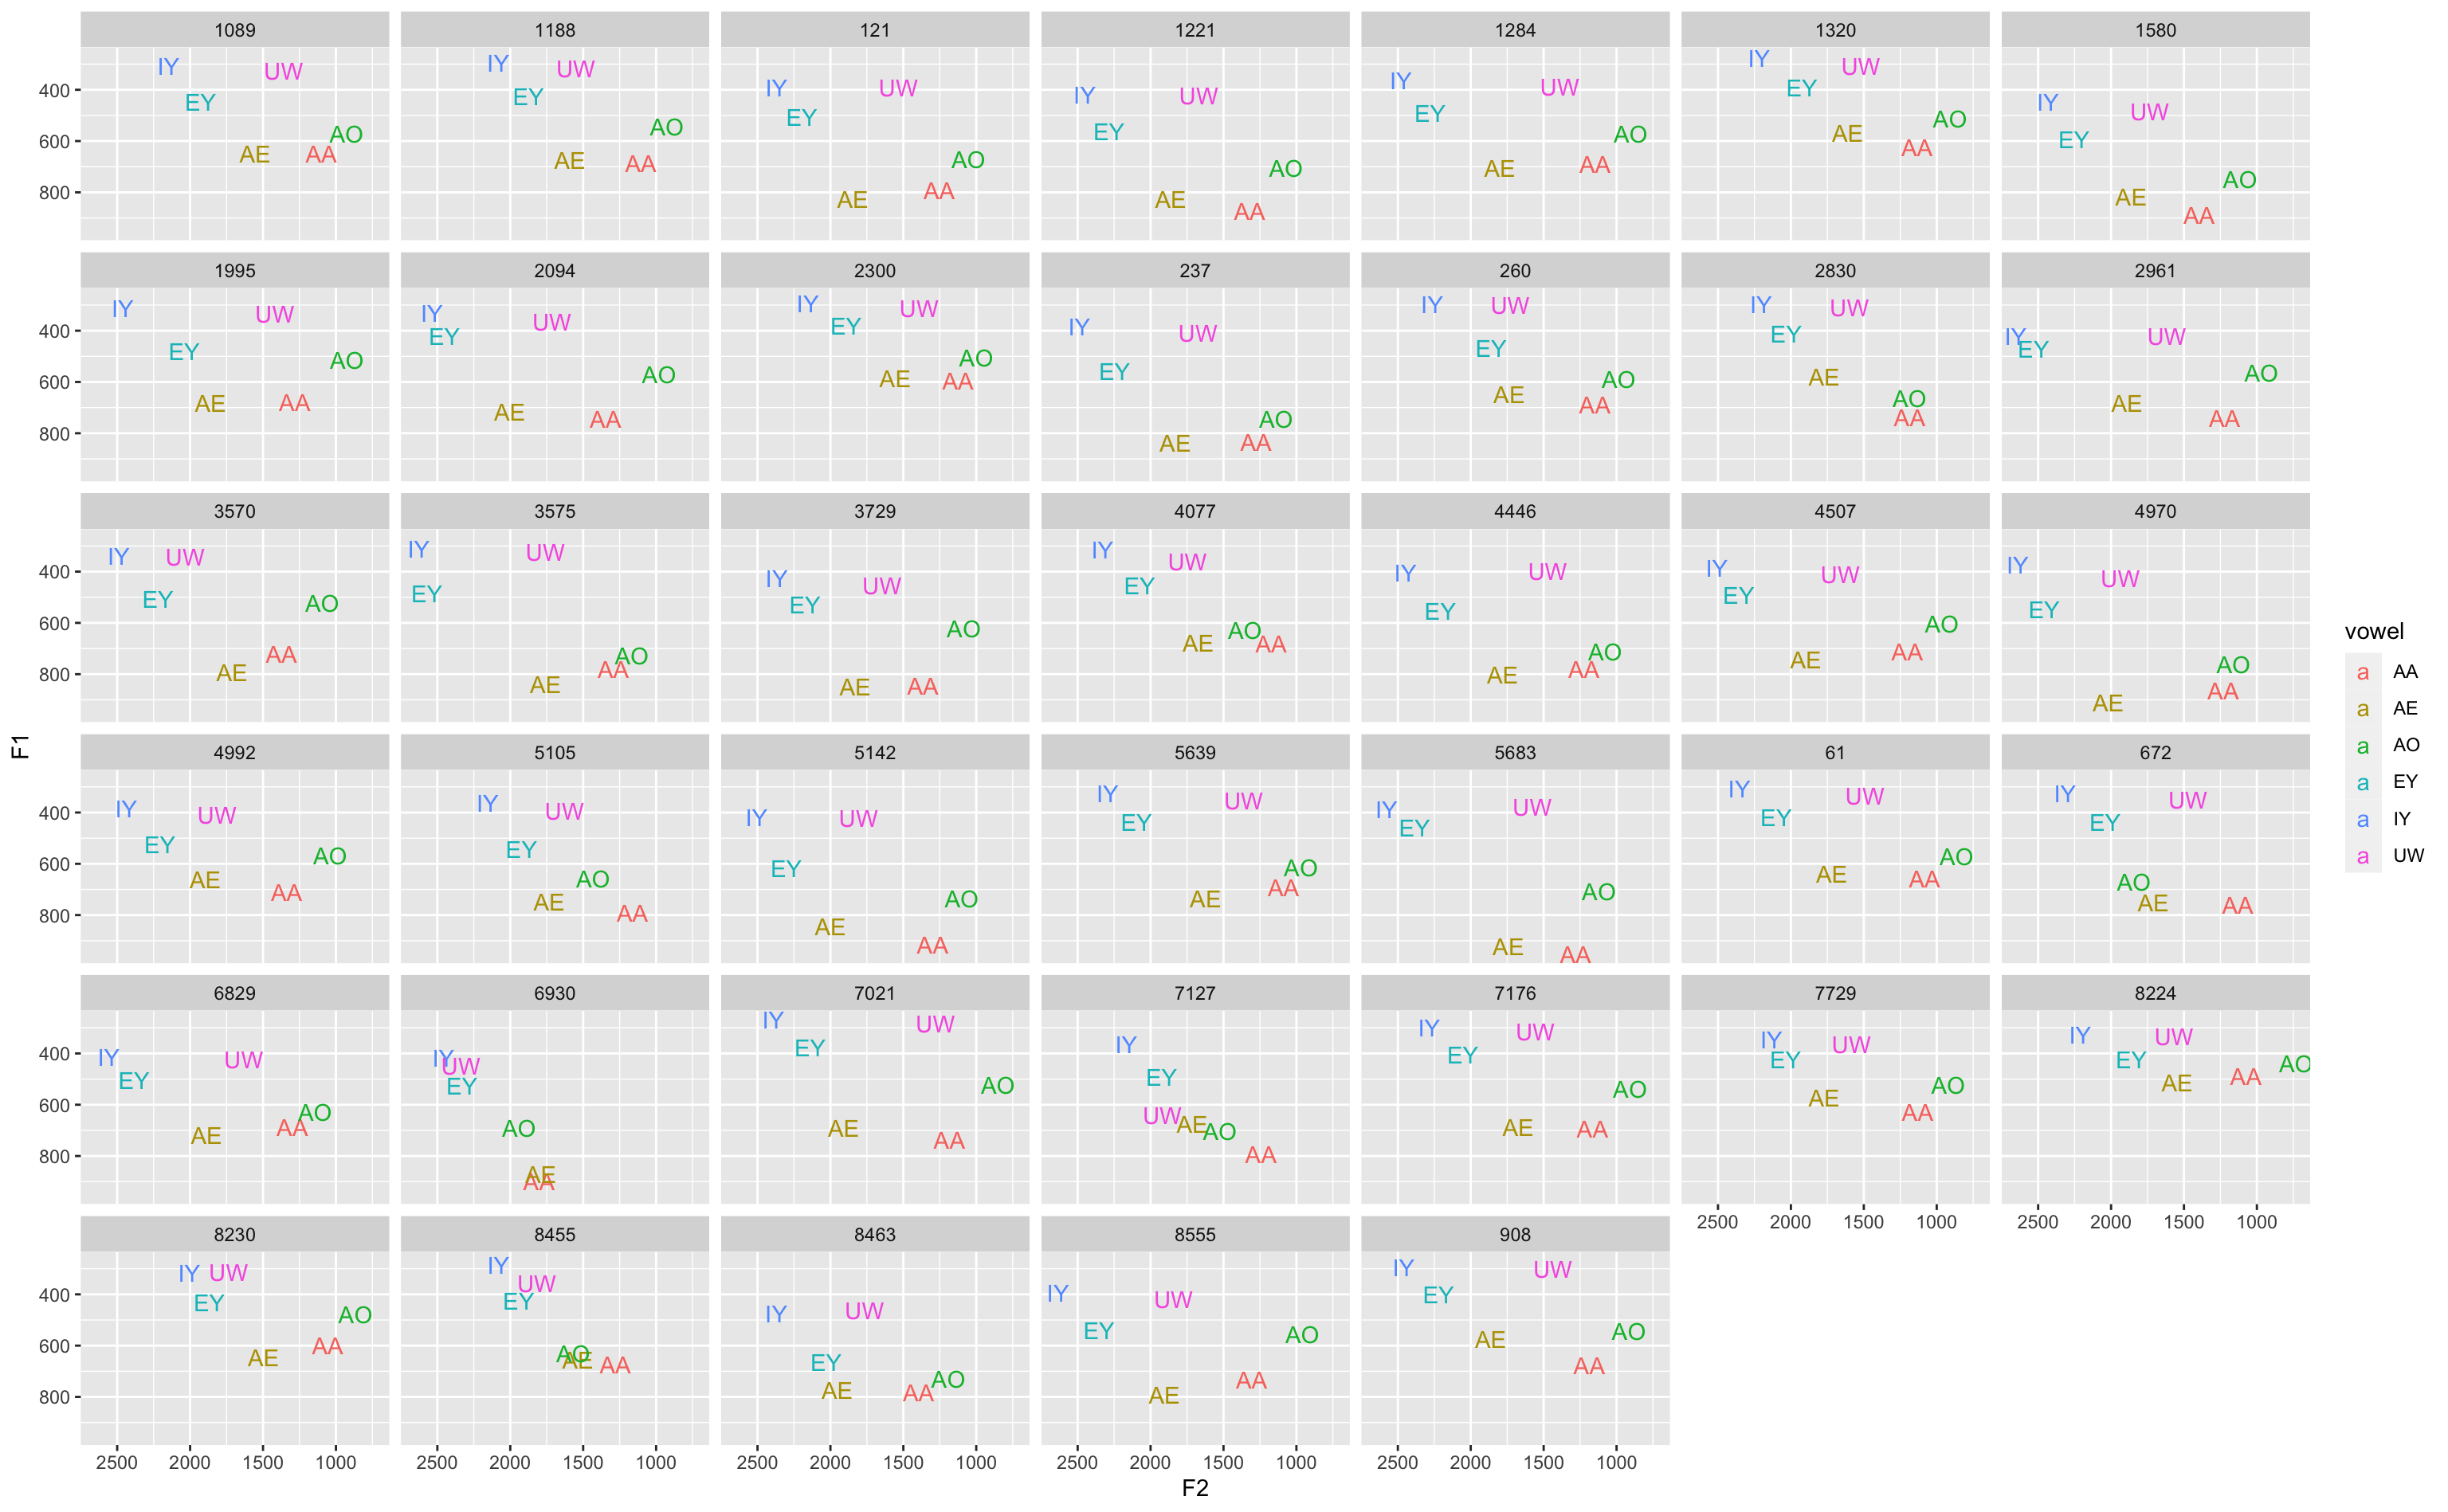
\includegraphics[scale=0.15]{dialect-analysis.png}
      \caption{The ``Cot--caught merger" is a well-known drift in some English dialects, particularly American English. In this graph, we can measure the vowel space distance between AO (``caught") and AA (``cot") to determine which speakers have the cot--caught merger in their dialect. For example, speakers such as 237, 2830, and 6829 may have AO == AA, indicating a merge, while speakers 1221, 2094, and 8555 may have distinct AO and AA. Figure produced using code written by Morgan Sonderegger (McGill).}
      \label{fig:dialect-analysis}
    \end{figure}

We can see that the Polyglot database we enriched can be used to address basic linguistics research questions -- and these are just the tip of the iceberg. The following section indicates areas of future work, which could be done on this corpus, or any other force-aligned speech data corpora.

\subsection{Future Work}

The following tasks, some taken up partially, others planned but abandoned to project scoping, would be interesting lines of research using the tools and methods established in this report:

\begin{itemize}
  \item As indicated in a previous section, completing the setup for PolyglotDB to be made available on condaforge would more reliably support this type of research on a wider array of development architectures
  \item The IARPA Babel corpora set has many other languages documented aside from Cantonese and Lithuanian. Languages such as Mixtec, Totonac, Yoruba, and Burmese in the IARPA Babel set is also more easily available for this type of research following the methods developed in this project.
  \item The Formant analysis performed in the previous section is just one example of an interesting linguistics question to investigate with corpora like these. Previous work has been done to demonstrate Pitch analysis\footnote{https://memcauliffe.com/playing-around-with-polyglotdb.html} using PolyglotDB, which provides further interesting data for analysis. These basic measurements open a wide range of research questions for amateur and expert researchers alike.
  \item Relatively more advanced linguistic analysis research could be performed with data sets like these, or even more general speech aligned data sets. One such question of particular interest to the author would be investigation into time-differentiated data sets to measure dialect change in time.
  \item A bit more speculative, but is certainly more room for automated software tools and paradigms for speech data sets. Word-vector analysis has seen incredible results in text-data natural language processing, and a similar paradigm applied to general speech-data corpora could see similar results.
\end{itemize}

\section{Software Design}
This section is a technical description of the software contributed to this project. The set of requirements covered in previous sections constitute a dynamic and varied set of requirements for such a system that can generalize to future corpora. These complications necessitate software design. The code written for this project made use of practices and principles like the Emergent Design Principle \cite{bain_emergent_2008}. These practices and principles are important in development generally, given that software requirements are always in a state of change, but are particularly important to this project where a major part of the utility of the software is to save time adapting its purposes to new corpora and new languages. 

This section will explain where relevant design principles were applied to the code base to aid future users and developers in generalizing the software to new contexts. This section will be of particular interest to developers who wish to extend the functionality of the software contributed, for example, to extend the number of languages supported for alignment preparation.

We saw in previous sections that speech data corpora vary in format. Character bounds between words, pronunciations, syllables, and phonemes can vary, in fact even between corpora published by the same author (we observed this with the IARPA Lithuanian and IARPA Cantonese corpora). Furthermore, various properties of languages can vary in predictable ways: languages will have different sets of characters for important lexical properties like vowels, sonorants, and tone markers. These sets of variations can all be encapsulated in a single data class, as shown in the figure below:

\begin{figure}[h]
\centering
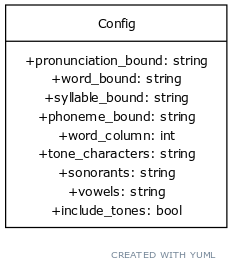
\includegraphics[scale=0.5]{config-uml.png}
\caption{A UML diagram of the Config class used to abstract common features that vary across corpora in the syllabify system.}
\label{fig:config-uml}
\end{figure}

Configurations are implemented as \verb|.yaml| files in this project. The configuration for the IARPA Cantonese corpus, for instance follows:

\begin{singlespace}
  \begin{verbatim}
    pronunciation_bound: "\t"
    word_bound: ""
    syllable_bound: " . "
    phoneme_bound: " "
    word_column: 1
    tone_characters: `_[0-5]'
    sonorants: ""
    vowels: "aeoiu69"
    include_tones: true
  \end{verbatim}
\end{singlespace}

These configuration files allow for variation in high level abstract properties of corpora without the need to known anything about the underlying implementation of the code. This is useful for two reasons: to prevent new code from needing to be written for new corpora, and to make the addition of new corpora easier for researchers who are not familiar with programming themselves.

Variation between corpora does not end, however, with changes in the format of the file nor simple properties of languages. We also saw in previous sections, particularly the \hyperlink{section.24}{Pronunciation Dictionary Production} section, that variation between languages and corpora is also observed in determining syllabic units for data representation. These variations are high-level abstractions themselves, more complicated than in-order processing: for one example, there is no inherent ordering to where tone makers are placed, as seen with the IARPA Cantonese and IARPA Lithuanian corpora. The method for which the syllabic units nucleus, coda, onset and tone are determined from language necessitates higher-order logic than configurational variation.

One way we can consider this problem is that there is a single behavior, "syllablify", that is common across all corpora. This ``syllabify" behavior should varying in implementation between corpora, but across corpora should have a common interface (a word/pronunciation pair) and reliably decompose the pronunciation into syllabic units so that these units can be used to produce uniform output. Moreover, we would like to decouple clients of this behavior from any one implementation -- at runtime, they should be able to specify which implementation without having to change any code. Finally, developers of the software should not have to change anything about the ``syllabify" interface and usage in order to add new implementations. 

These requirements naturally evoke the Strategy pattern\cite{freeman_head_2004}, a classic behavioral pattern for allowing variation in algorithm to be encapsulated by a generic Strategy class.

\begin{figure}[h]
\centering
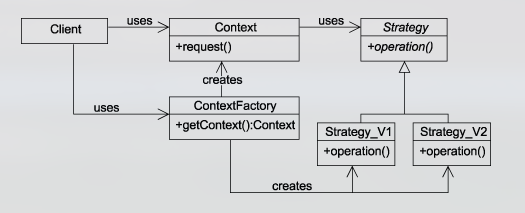
\includegraphics[scale=0.5]{strategy-pattern.png}
\caption{The variation of the Strategy Pattern used in this project, with creational logic is encapsulated in a factory class. Generic classnames shown here (e.g. Strategy) are specified in the following figure. Source: Figure B.54 in Bain, 2008\cite{bain_emergent_2008}}
\label{fig:strategy-pattern}
\end{figure}

\begin{figure}[h]
  \centering
  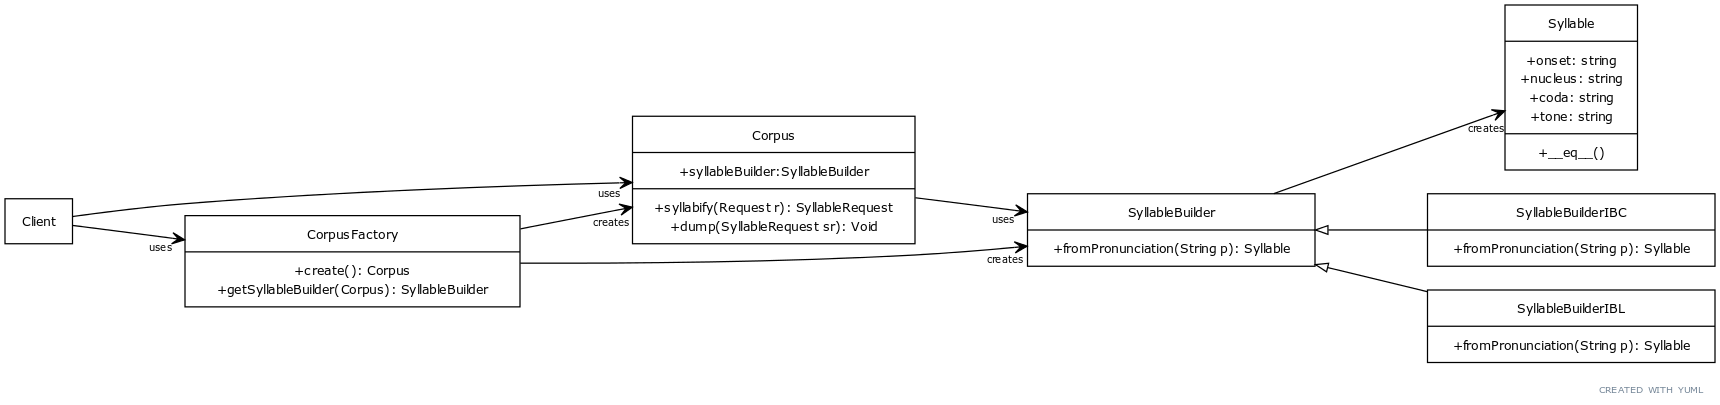
\includegraphics[scale=0.25]{syllabify-pattern.png}
  \caption{The actual pattern implemented for the syllabify system developed for this project, with some classes redacted to make the pattern clearer. See the Appendix, Section 6.1 for the full UML diagram. The SyllableBuilder classes stand in as the variable strategies: adding linguistic support for building syllables for a new corpora only involves creating another SyllableBuilder subclass, without modifying any part of the rest of the system.}
  \label{fig:syllabify-pattern}
\end{figure}

The design is encapsulated and extensible because ``the various versions of the behavior, how many variations there are, which variation will be used under a given circumstance, and the design of each varying implementation are all hidden from the client"\cite{bain_emergent_2008}. That is, the varying corpora language properties and format distinctions for speech-data experiments can be abstracted to algorithms that are variable at run-time, decoupled from the generic behavior required to ``syllabify", and easily extensible to development in the future.

Further details about design choices are elaborated in a complete UML diagram of the syllabify system in the \hyperlink{section.6}{Appendix, Section 6.1}.

\section{Conclusions}

This report outlined some novel complications introduced by the adaptation of speech-text corpora varying across language and formatting conventions for concrete linguistic analysis. While tools exist for the preparation problems of corpora storage and speech-text alignment, there remains manual scripting involved to adequately create a development environment for interesting linguistic research. This project developed a procedure, applied to two corpora of varying format and language, which enabled automation in the preparation of speech corpora for forced-alignment, as well as the procedure for performing basic linguistic analysis on aligned speech corpora.

This procedure surrounds the automation of various steps in corpora preparation: corpora acquisition and normalization, transcript encoding, audio signal processing, and lexicon convention generalization. While many of these variations can be abstracted to configuration, parsing lexicon files to create phonetically valid data representations for conversion between formats proved to be a high-level abstract which required designed software to perform reliably. The software contributed in this report aims to fill just that gap: to provide automation general enough to extend to corpora varying in language and format, to further the accessibility of research on corpora requiring alignment.

This required generalization is accomplished by abstracting differences between corpora to both configuration and to a Strategy pattern-based python library. Using this approach, new corpora can be supported by modifying a template configuration file and adding a single subclass, rather than modifying existing scripts or code. The software developed to perform this task is made available for study, use, and extension in a public repository.

The upshot of corpora preparation was also analysed in this report. Experiments demonstrating the usage of PolyglotDB with similar corpora verified known experimental results in order to show that investigation into interesting linguistic questions, namely: (1) formant frequency aggregated across a large sample of speakers, and (2) dialect feature detection through measurement of variation in pronunciation across a large sample of speakers.can be attained and the procedure for preparation automated across corpora, is possible with existing speech-text software tools.

Some of the aims set at the outset of the project were not reached: the procedure developed here invites investigation and publication of research into even more profound linguistic questions that can be studied through publicly available corpora beyond Librispeech. This report outlined some possible avenues for future work, as well as some suggested improvements to the software contributed in this project.

These are humble and imperfect contributions, but hopefully they can play a role in the extension of engaging speech data corpora research.


\subsection{Acknowledgments}

The completion of this report would have been impossible without the support of my supervisor Morgan, my advisor Ann, my mentor Jasmine, my partner Ma\"ia, and many cherished family, colleagues, comrades, teachers, and friends who are invaluable parts of my life and have uplifted me in innumerable ways along the long way.

\newpage
\section{Appendix}
\subsection{Syllabify System UML Diagram}
\begin{figure}[h]
  \centering
  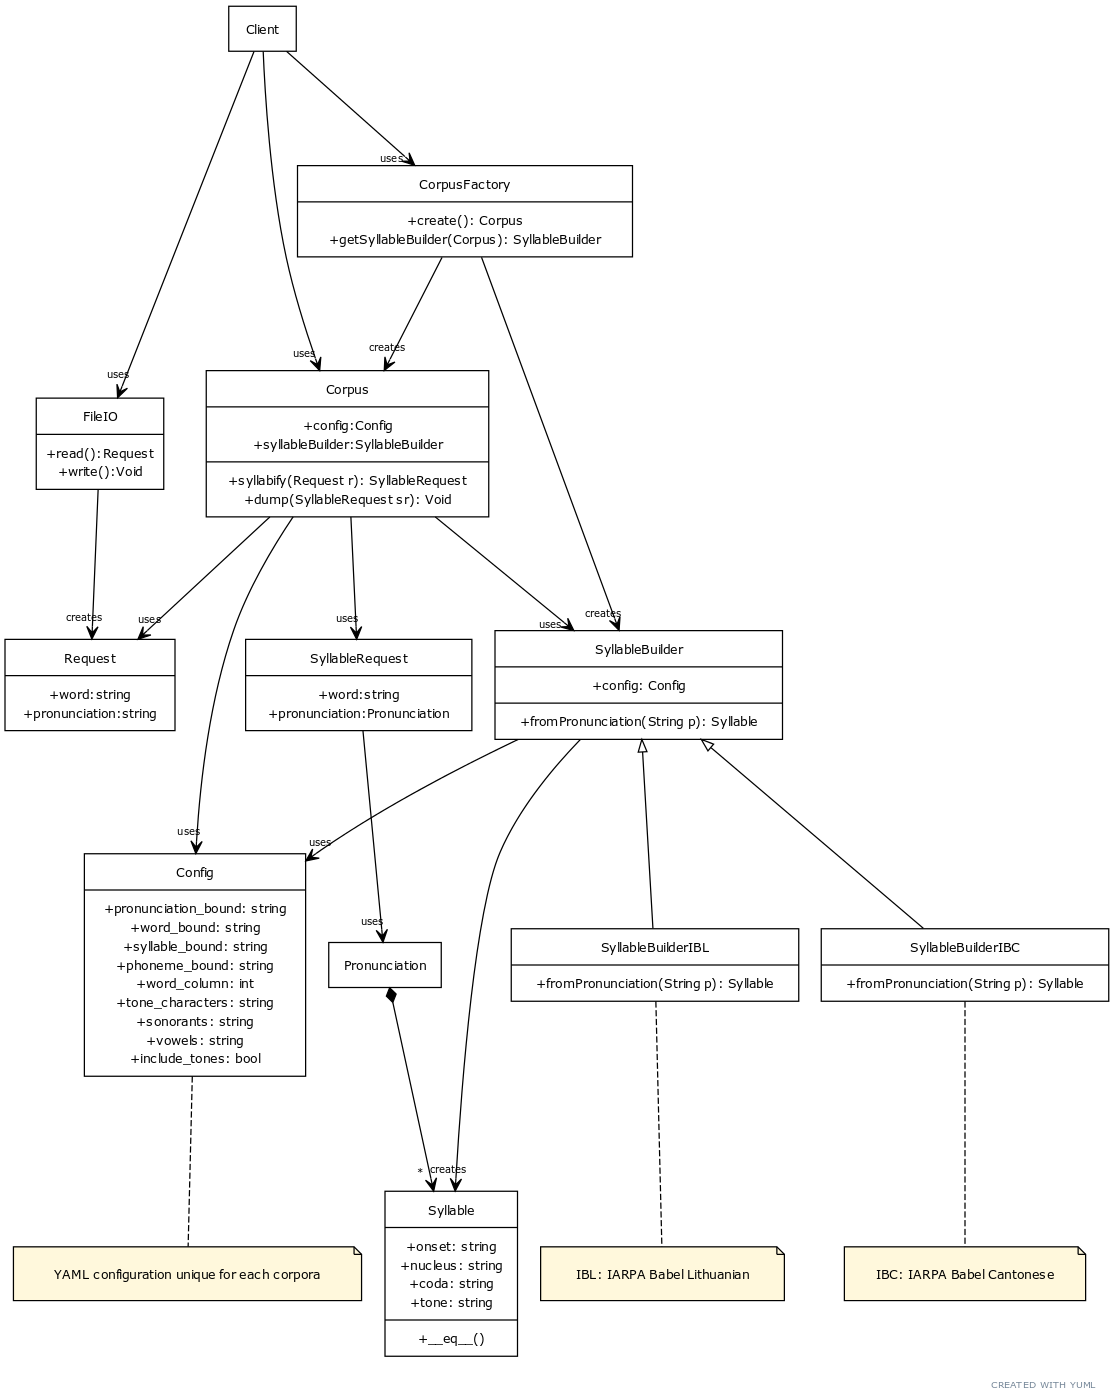
\includegraphics[scale=0.3]{UMLdiag.png}
  \caption{The complete UML diagram for the syllabification system produced during this project. The Strategy Pattern components can be seen in the Corpus/SyllableBuilder/Client relationships: the client can choose syllabification at runtime using configuration (for elements common to all languages) and dynamic algorithmic support (for elements unique to each language requiring higher-order logic) provided by the pattern.}
  \label{fig:UMLdiag}
\end{figure}

\newpage

\vskip 0.2in
\bibliographystyle{unsrt}
\bibliography{sample}

\end{document}
